\documentclass[a4paper,12pt]{article}

\usepackage[utf8]{inputenc}
\usepackage[T1]{fontenc}
%\usepackage{ngerman}
\usepackage[hidelinks]{hyperref}
\usepackage{graphicx}
\usepackage[font=footnotesize]{caption}
\usepackage{amsthm,amsmath,amsfonts}
               
\newtheorem{theorem}{Theorem}
\newtheorem{lemma}{Lemma}
\newtheorem{definition}{Definition}
%\renewcommand{\proofname}{Beweis}

\usepackage{lineno}

               
\title{My Topic XYZ\\
	\emph{Seminar: Foundations of Data Science}}
\author{%Stefan Mustermann, Matr.-Nr.:12345\\
	%Fakultät Statistik/Informatik\\
	Jane Public, enrolment no.: 12345\\
	Faculty of Statistics / Computer Science\\
	TU Dortmund
	}

\date{\today\\%im WS
	winter term 
	2020/21}

\begin{document}
\maketitle
\linenumbers
\begin{abstract}
%Eine kurze Zusammenfassung von etwa zwei bis drei Sätzen, die den Inhalt kurz und prägnant umreißen \ldots
A short summary of about two to three sentences that briefly and concisely outline the content \ldots
\end{abstract}

\section{%Einleitung
		Introduction}
%In dieser Arbeit geht es um die Grundlagen der Datenwissenschaften. Wir beschäftigen uns speziell mit dem Thema XYZ, welches sehr vielseitig ist und neben der theoretischen Tiefe auch viele praktische Anwendungen hat.
This article deals with the fundamentals of data science. We are covering the topic XYZ in particular, which is very interesting and besides the theoretical depth has many practical applications.


%Wir beginnen mit einer Definition, die eine zentrale Rolle in dieser Arbeit spielt.
We start with a definition, which plays a central role in this work.
\begin{definition}{%(Euklidische Norm)}
				(Euclidean norm)}
\begin{linenomath*}
	%Sei $x\in\mathbb{R}^d$ dann bezeichne $$\|x\|=\sqrt{\sum_{i=1}^{d} x_i^2}$$ die Euklidische Norm von $x$.
	Let $x\in\mathbb{R}^d$. We denote by $$\|x\|=\sqrt{\sum_{i=1}^{d} x_i^2}$$ the Euclidean norm of $x$.
\end{linenomath*}
\end{definition}
	
\section{%Hauptteil
	Main Part}
\label{main_part}
%Hier arbeiten wir mit den obigen Definitionen und Notationen und leiten wichtige Ergebnisse her, wie beispielsweise den folgenden Satz über die kleinste-Quadrate-Lösung.
Here we work with the above definitions and notations and derive important results such as the following Theorem on the least-squares solution
\begin{theorem}{%(Nützlicher Satz)}
		(useful theorem)}
\label{thm:main}
\begin{linenomath*}
	%Seien $X\in\mathbb{R}^{n\times d}, Y\in\mathbb{R}^n$ und sei $\beta^* = \operatorname{argmin}_{\beta\in R^d}\|X\beta-Y\|^2$. Dann gilt $$\|Y\|^2=\|X\beta^*\|^2 + \|X\beta^* - Y\|^2.$$
	Let $X\in\mathbb{R}^{n\times d}, Y\in\mathbb{R}^n$. Further define $\beta^* = \operatorname{argmin}_{\beta\in R^d}\|X\beta-Y\|^2$. Then $$\|Y\|^2=\|X\beta^*\|^2 + \|X\beta^* - Y\|^2.$$
\end{linenomath*}
\end{theorem}
\begin{proof}
	%Der Beweis verbleibt als Übungsaufgabe.
	The proof is left as an exercise.
\end{proof}

\begin{figure}[t!]
	\centering
	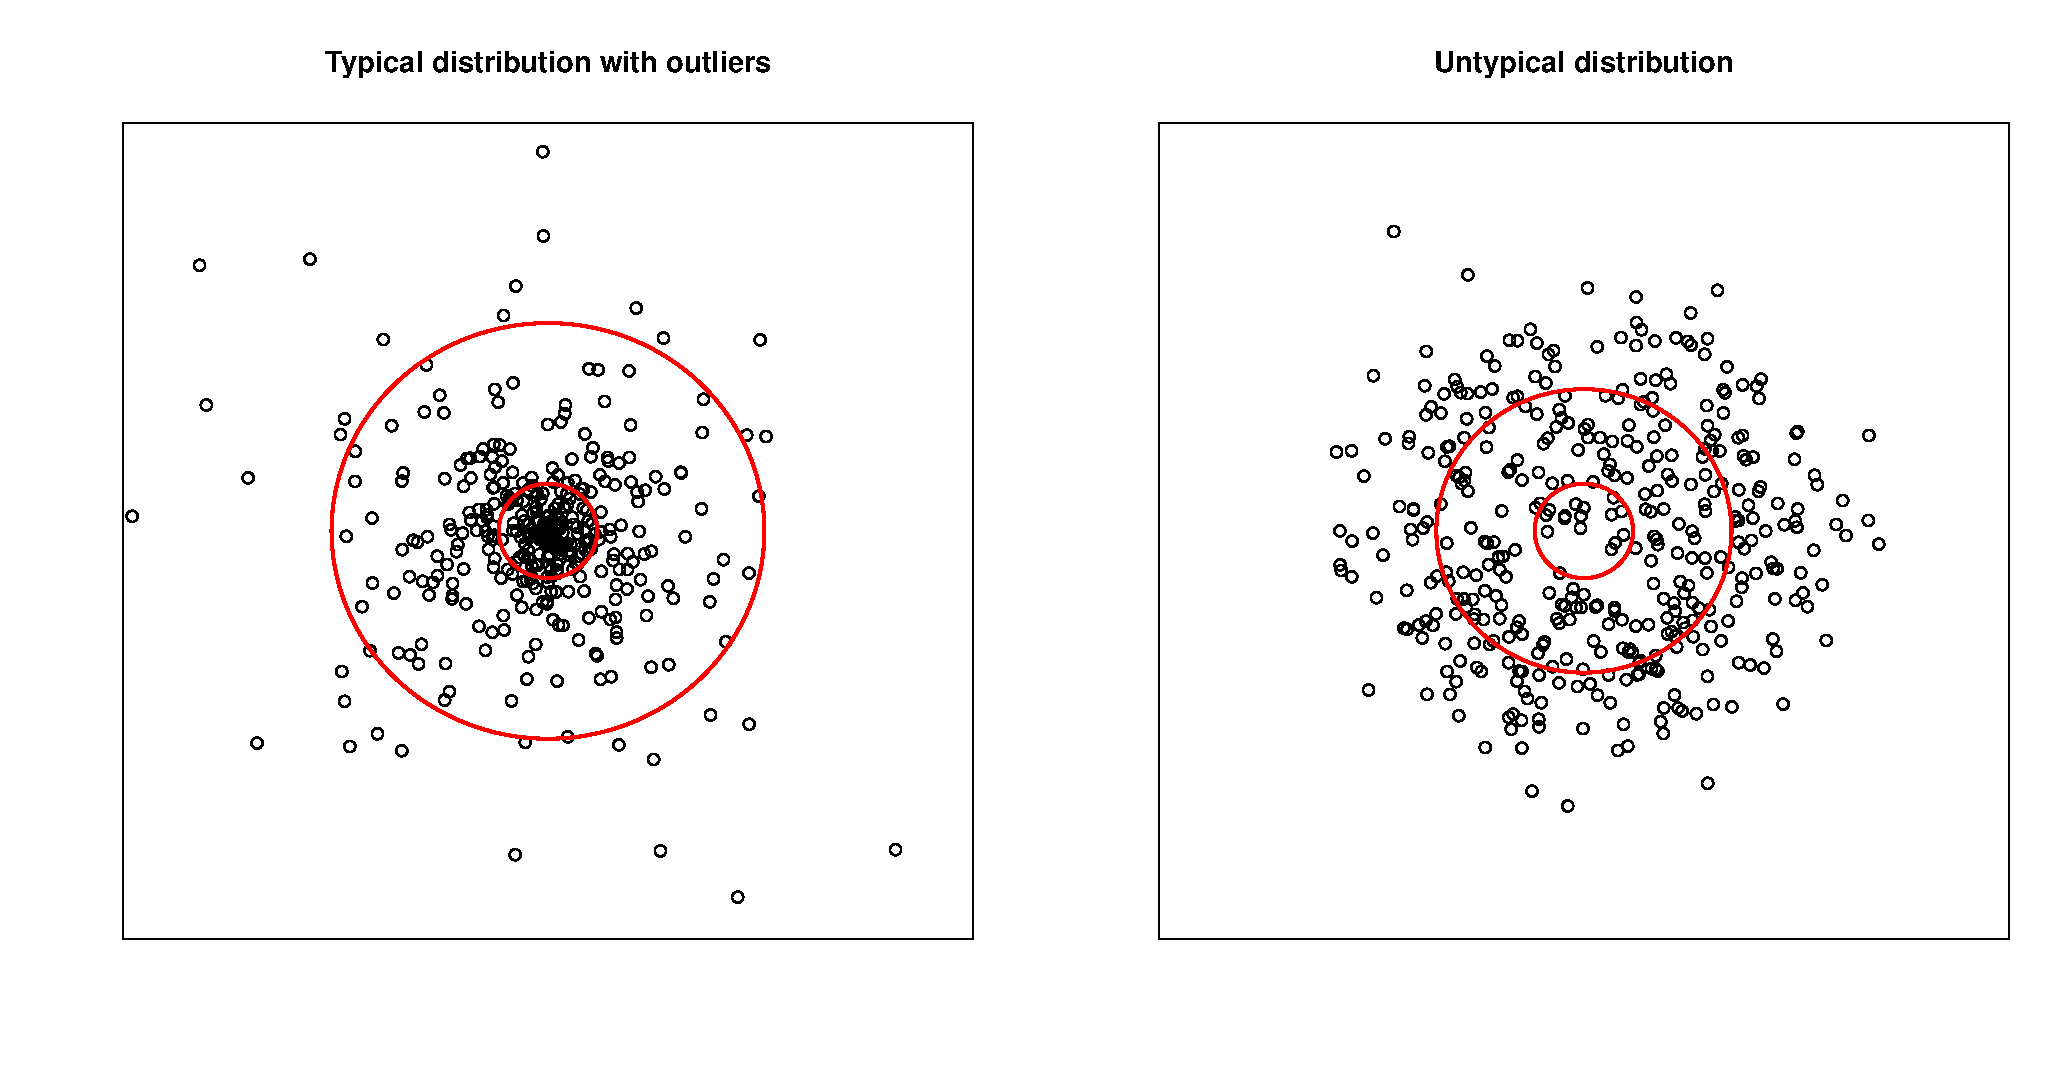
\includegraphics[width=\textwidth]{median_distr}
	%\caption{Verteilungen von Punkten um ihren Median zentriert. Die Caption steht gerne unter der Grafik.}
	\caption{Distributions of points centered around their median. The caption should be placed below the figure.}
	\label{fig:median_distr}
\end{figure}


%Manchmal hilft eine Grafik zur anschaulichen Verdeutlichung von Formalismen. Abbildung~\ref{fig:median_distr} zeigt ein Beispiel aus der Analyse von Samplingalgorithmen zur Approximation des geometrischen Median, was unpassender weise nichts mit Theorem~\ref{thm:main} zu tun hat.
Sometimes figures help to illustrate a formalism. Figure~\ref{fig:median_distr} shows an example from the analysis of sampling algorithms for approximating the geometric median, which inappropriately is completely unrelated to Theorem~\ref{thm:main}.

\section{%Fazit
	Conclusion}
\label{conclusions}
%Nach langer Forschung im Bereich der Datenwissenschaften hat sich nichts vielseitigeres ergeben als der nützliche Satz aus Kapitel~\ref{main_part}. Er findet überall Anwendung und hat zu den tollsten und kühnsten Resultaten geführt, vgl. \cite{Someone03}. Übrigens ist das Buch zum Seminar \cite{BlumHopcroftKannan20} ein tolles Nachschlagewerk und darf gerne referenziert werden. Weitere Literaturhinweise finden sich in den jeweiligen \emph{bibliographic notes} und dürfen natürlich auch selbst recherchiert und ergänzt werden.
Even after centuries of research in the field of data science, there is nothing more versatile than the useful theorem of chapter~\ref{main_part}. It is used everywhere and has led to the greatest and most intriguing results, cf. \cite{Someone03}. By the way, the book for the seminar \cite{SSBD14} is a great reference and should be cited. Further literature can be found in the respective \emph{Bibliographic Remarks} sections and of course you are welcome to search and add your own references.

%\paragraph*{Anmerkung:} Literatureinträge sind häufig in der Sammlung DBLP zu finden. Auch Google Scholar bietet Bib\TeX~Einträge, die in die .bib Datei kopiert werden können und ggf. geringfügig angepasst werden müssen.
\paragraph*{Note:} Bib\TeX~entries entries can often be found in the DBLP collection. Google Scholar also offers Bib\TeX~entries, which can be copied into the .bib file and may need some minor adjustments.
\bibliographystyle{abbrv}

\nolinenumbers
\footnotesize
\bibliography{bibliography}
\end{document}